%%%%%%%%%%%%%%%%%%%%%%%%%%%%%%%%%%%%%%%%%%%%%%%%%%%%%%%%%%%%%%%%%%%%%%
%%                    Non-Interaction
%%%%%%%%%%%%%%%%%%%%%%%%%%%%%%%%%%%%%%%%%%%%%%%%%%%%%%%%%%%%%%%%%%%%%%
\color{red}

\subsubsection{Glyph: \glyph{Non-Interaction}}\label{sec:non-interaction}

\glyph{Non-interaction} represents the absence of an interaction between two or more \glyph{entities} or \glyph{outcomes}, whether a non-covalent physical interaction, or a functional interaction, e.g. genetic interaction. Each arrowhead points to an interactor involved in the absent interaction. The result of the non-interaction is represented by \glyph{outcomes} (see section \ref{sec:outcome}), that is by filled dots on the line linking the two arrowheads in the case of a binary interaction, on a circle linked to the edges coming from the arrowheads in the case of a  n-ary interactions. The result of an interaction can be represented by any number of \glyph{outcomes}.

\begin{glyphDescription}
 \glyphSboTerm SBO:NEW
 \glyphOrigin Any \glyph{interactor} (\sect{interactors}).
 \glyphTarget Any \glyph{interactor} (\sect{interactors}).
 \glyphEndPoint Both origin and target extremities of an \glyph{interaction} carry an harpoon arrowhead. The absence of the interaction is denoted by two parallel bar perpendicular to the arc.
 \end{glyphDescription}

\begin{figure}[H]
  \centering
  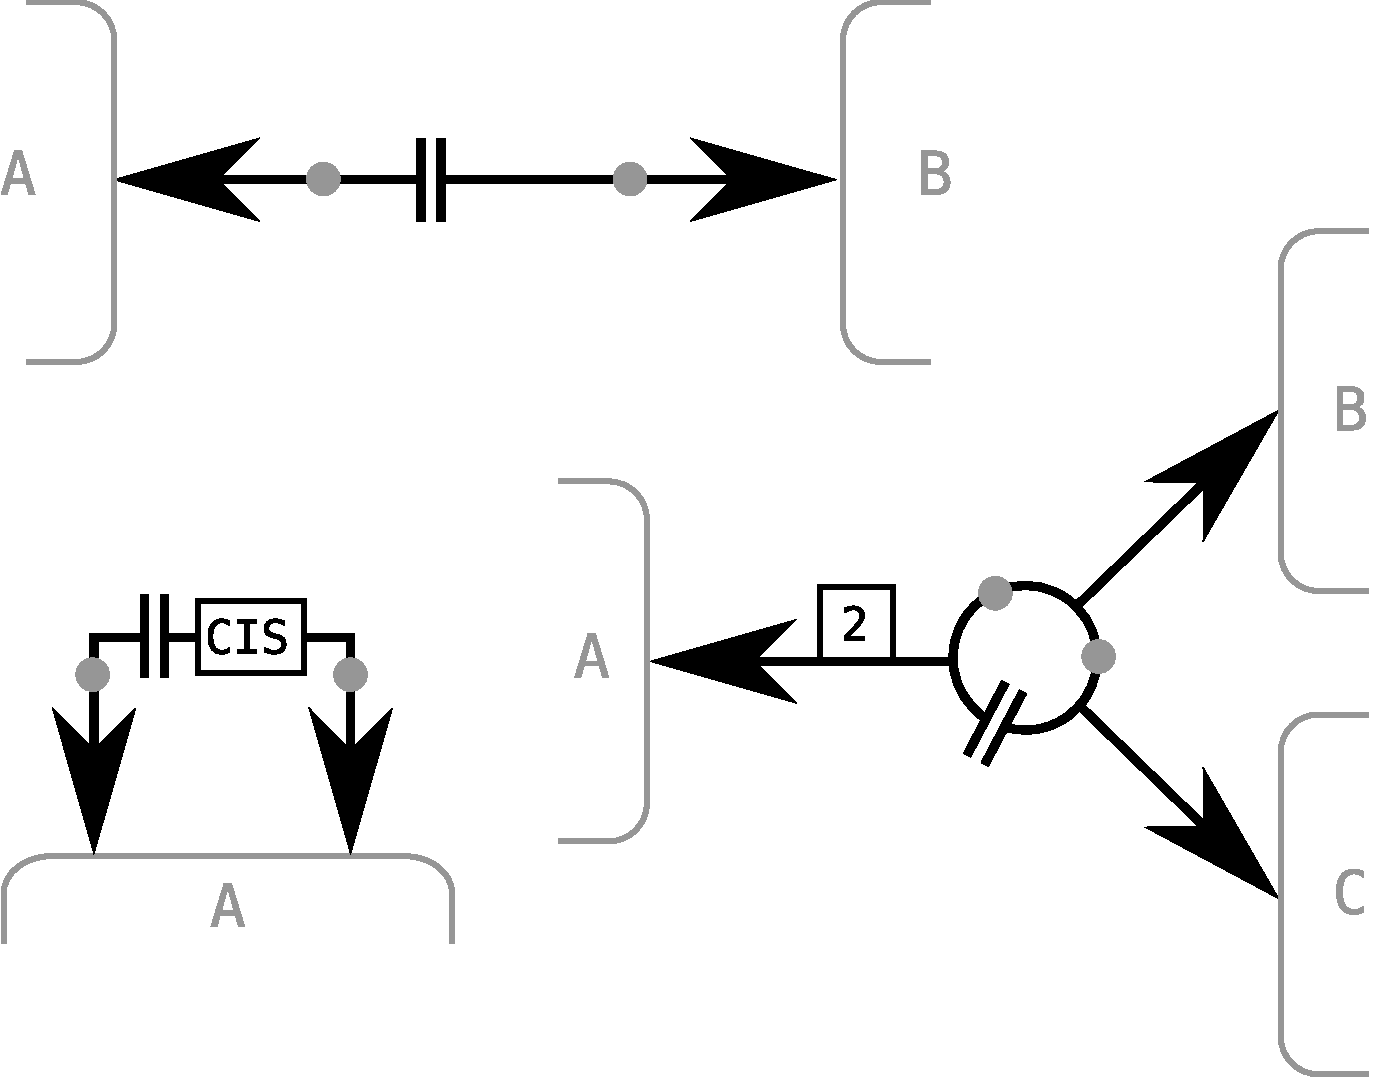
\includegraphics[scale = 0.3]{images/non-interaction}
  \caption{The \ER glyph for \glyph{non-interaction}. Top, binary interaction; bottom, n-ary interaction.}
  \label{fig:interaction}
\end{figure}
% 
% \begin{figure}[H]
%   \centering
%   \includegraphics[scale = 0.5]{examples/ex-interaction}
%   \caption{Examples of \glyph{interactions}. The interaction between calcium and Calmodulin influences the interaction between Calmodulin and CaMKII.}
%   \label{fig:ex-interaction}
% \end{figure}

%%% Add a part on cis- versus trans-interactions

%%% Add a part on cardinality, with an example of alternative interactions with different cardinalities.

\normalcolor